\section{Experimental Results}
\ifCLASSOPTIONonecolumn\begin{figure*}[t]
\centering
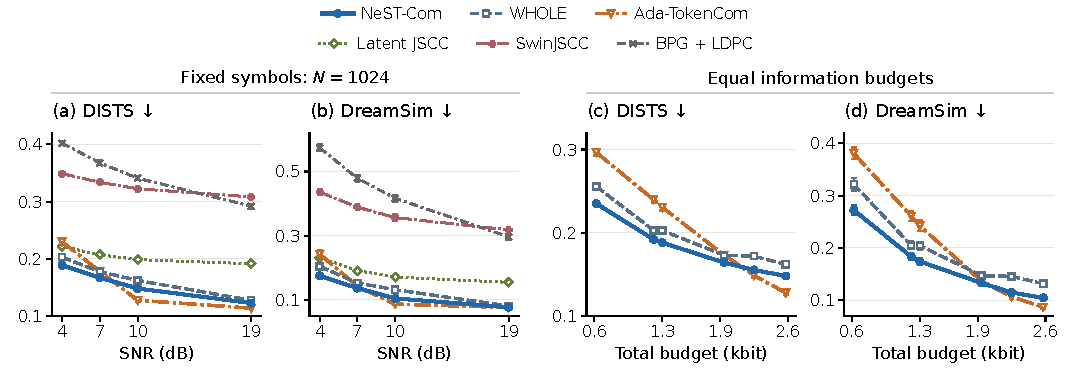
\includegraphics[width=\linewidth]{figure2_1x4.pdf}
\caption{Source-referenced reconstruction on 500 ImageNet images. (a,b) Six methods at $N=1024$; WHOLE, NeST and Ada share the 12-MCS calibration procedure. Three outcomes per source include gray failures. (c,d) Equal, error-free information budgets pay 57 shared protocol bits and Ada's additional 10-bit class; WHOLE/NeST share ceiling $(10,0)$. Points and bars are equal-source means and pointwise 95\% source-bootstrap intervals after within-source averaging. Ada-TokenCom is the predicted-class, fixed-frame adaptation. Lower values are favorable.}
\label{fig:performance}
\end{figure*}
\fi
\subsection{Setup and Calibration Protocol}
We evaluate 500 ImageNet validation images~\cite{imagenet} at $256\times256$, disjoint from 1000 calibration images, across $N=1024$ (4/7/10/19 dB) and $N=512$ (4/10/19 dB). After averaging three channel realizations per image (retaining gray failures), we report equal-source means and paired 95\% intervals from 10\,000 source-bootstrap resamples. Matched controls use the first 100 test images; token systems share noise realizations, while external baselines retain their own noise.

Among baselines, Latent JSCC maps tokenizer latents to symbols and shares $\Dc$ (MSE, LPIPS, and latent-consistency losses, 100k updates), whereas SwinJSCC~\cite{swinjscc} trains with RGB MSE (200k updates, calibration-MSE selection); both use 20\,000 training images at $N=1024$. BPG~\cite{bpg} is paired with 5G NR LDPC/QAM. Ada-TokenCom~\cite{adatokencom} is adapted to fixed frames without ARQ or long-term queues using LlamaGen-L/VQ16, prefix arithmetic coding, $\mathrm{CFG}=4$, $T=1$, top-$k=2000$, top-$p=1$, and a paid 10-bit ConvNeXt class.

We evaluate DISTS~\cite{dists}, DreamSim~\cite{dreamsim}, PSNR, LPIPS-Alex~\cite{lpips}, and CLIP-I~\cite{clip} on native float RGB. GPU-synchronized TX (RGB-to-symbols) and RX (symbols-to-RGB) latencies are measured over 32 images (batch one, two warmups, three runs) on one RTX PRO 6000 with two physical CPU cores, covering coding, link processing, and generation while excluding I/O and scoring. Supplementary Sections~S2--S4 provide extended controls, timing, transfer tests, and ARPC's protected digital-link adaptation.

All transmit policies are calibrated once and frozen. At $N=1024$, WHOLE, NeST, and Ada share 12 MCSs (QPSK/16-QAM/64-QAM at rates $1/2, 2/3, 3/4, 5/6$), with seven complete-scale ceilings for WHOLE, 25 Quarter ceilings (with Token fallback) for NeST, and a 256-token ceiling for Ada. All 396 candidates are screened on a 100-image pilot; per method and SNR, the top three plus a preset QPSK rate-$1/2$ anchor are evaluated on all 1000 calibration images (three realizations), selecting the policy maximizing mean DINOv2 cosine~\cite{dinov2} including gray failures. Policies for $N=512$ are calibrated independently under the same protocol, with public profile directories fixed prior to calibration.

\begin{table}[t]
\caption{Within-scale transmission. (A) Ordered receiver interventions. (B) Shared-model NeST--WHOLE differences. (C) Matched endpoint granularity. Brackets are source-paired 95\% intervals; sample sizes are specified for each block.}
\label{tab:internal}\centering\footnotesize
\setlength{\tabcolsep}{2.1pt}\renewcommand{\arraystretch}{1.05}
\begin{tabular}{@{}lccc@{}}\toprule
\multicolumn{4}{l}{\textit{A. 100 sources, 10 dB, same received prefixes}}\\
Intervention & $\Delta$PSNR (dB) & $\Delta$DISTS & $\Delta$DreamSim\\
\midrule
B0--A0 & \shortstack{+0.287\\{}[0.240, 0.335]} & \shortstack{-0.0062\\{}[-0.0077, -0.0048]} & \shortstack{-0.0113\\{}[-0.0147, -0.0083]}\\[2pt]
C0--B0 & \shortstack{+0.537\\{}[0.404, 0.682]} & \shortstack{-0.0083\\{}[-0.0102, -0.0065]} & \shortstack{-0.0159\\{}[-0.0205, -0.0116]}\\[2pt]
\bottomrule\end{tabular}
\par\smallskip
\begin{minipage}{\ifCLASSOPTIONonecolumn 3.4in\else\columnwidth\fi}\scriptsize
A0: prior completion without received boundary tokens. B0: A0 plus boundary residual correction. C0: B0 plus updated finer-scale conditioning.
\end{minipage}
\par\smallskip
\begin{tabular}{@{}lccc@{}}\toprule
\multicolumn{4}{l}{\textit{B. 500 sources, $N=1024$, uniformly calibrated policies}}\\
SNR & Util. W$\to$N (\%) & $\Delta$DISTS & $\Delta$DreamSim\\
\midrule
4 & 73.81$\to$99.56 & \shortstack{-0.0142\\{}[-0.0155, -0.0127]} & \shortstack{-0.0297\\{}[-0.0330, -0.0264]}\\[2pt]
7 & 83.19$\to$99.71 & \shortstack{-0.0103\\{}[-0.0139, -0.0068]} & \shortstack{-0.0159\\{}[-0.0207, -0.0112]}\\[2pt]
10 & 77.70$\to$99.79 & \shortstack{-0.0141\\{}[-0.0153, -0.0128]} & \shortstack{-0.0270\\{}[-0.0299, -0.0241]}\\[2pt]
19 & 85.24$\to$99.83 & \shortstack{-0.0048\\{}[-0.0053, -0.0043]} & \shortstack{-0.0043\\{}[-0.0051, -0.0036]}\\[2pt]
\bottomrule\end{tabular}
\par\smallskip
\begin{tabular}{@{}lrrrr@{}}\toprule
\multicolumn{5}{l}{\textit{C. 100 quality sources; 32 timing sources; ceiling $(8,126)$}}\\
Grid & Util. (\%) & DISTS & DreamSim & TX (ms)\\\midrule
Whole & 78.13 & 0.1650 & 0.1387 & 185.2\\
Quarter & 95.19 & 0.1535 & 0.1143 & 215.8\\
Eighth & 97.44 & 0.1516 & 0.1137 & 217.8\\
Token & 99.85 & 0.1505 & 0.1115 & 248.4\\
\bottomrule\end{tabular}
\end{table}

\ifCLASSOPTIONonecolumn\else\begin{figure*}[t]
\centering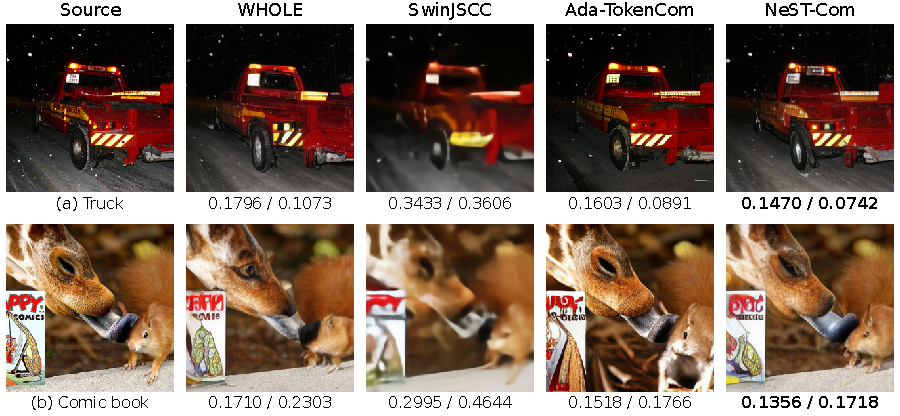
\includegraphics[width=6.0in]{figure3.pdf}
\caption{Selected reconstructions at $N=1024$ and 10 dB under the calibrated 16-QAM rate-$2/3$ policies (ceilings $(9,0)$, $(8,126)$, and $256$ tokens for WHOLE, NeST-Com, and the predicted-class fixed-frame Ada-TokenCom adaptation). Values are full-image DISTS$\downarrow$ / DreamSim$\downarrow$ for each method's first prescribed realization; sources were selected for favorable perceptual examples before recalibration.}
\label{fig:qualitative}\end{figure*}
\fi
\subsection{Within-Scale Fitting and Mechanism Attribution}
Block A in Table~\ref{tab:internal}(A) holds the received NeST prefixes fixed and intervenes solely at the receiver: A0 predicts boundary and finer maps without boundary tokens, B0 adds boundary residual correction under A0's conditioning, and C0 updates finer-scale conditioning with the merged map. At 10 dB, B0--A0 and C0--B0 yield $+0.287$ and $+0.537$~dB in PSNR, with paired intervals confirming gains on PSNR, DISTS, and DreamSim at both stages.

Table~\ref{tab:internal}(B) compares NeST and WHOLE under shared weights and family-calibrated policies; even when both select the same target ceiling (e.g., at 7 and 19 dB), high-entropy images exceeding capacity force WHOLE back to the preceding complete scale whereas NeST falls back within the scale. All five paired metrics favor NeST across all seven operating points. At $N=1024$ and 10 dB, source-bit utilization rises from 77.70\% to 99.79\%, reducing DISTS by 8.7\% ($-0.0141$) and DreamSim by 20.5\% ($-0.0270$; Fig.~\ref{fig:performance}(a,b) and Supplement Table~S4), while raising mean PSNR from 19.31 to 20.19~dB ($+0.88$~dB; Table~\ref{tab:external}).

Block C (Table~\ref{tab:internal}(C)) isolates endpoint granularity at fixed 16-QAM rate $2/3$ and ceiling $(8,126)$. Eighth captures roughly 92\% of the Whole-to-Token gains in PSNR, DISTS, and DreamSim at lower complexity, whereas Token lifts utilization from 97.44\% to 99.85\% with statistically significant paired gains at 14.1\% higher TX latency (Supplement Table~S3).

\subsection{System-Level Comparison}
\ifCLASSOPTIONonecolumn\begin{figure*}[t]
\centering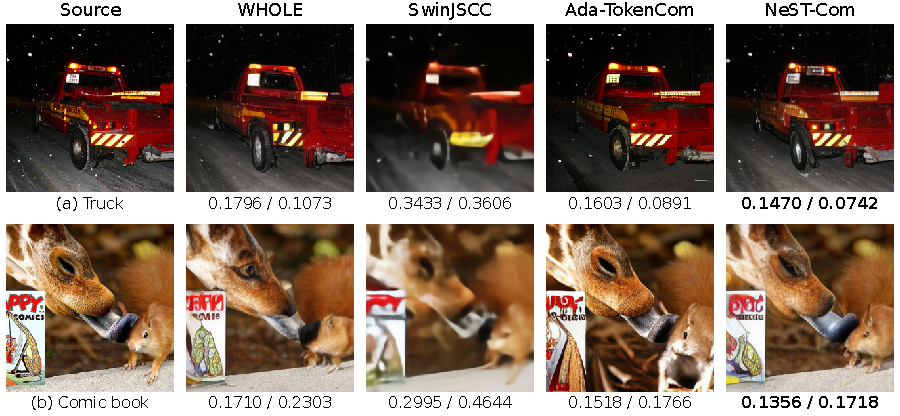
\includegraphics[width=6.0in]{figure3.pdf}
\caption{Selected reconstructions at $N=1024$ and 10 dB under the calibrated 16-QAM rate-$2/3$ policies (ceilings $(9,0)$, $(8,126)$, and $256$ tokens for WHOLE, NeST-Com, and the predicted-class fixed-frame Ada-TokenCom adaptation). Values are full-image DISTS$\downarrow$ / DreamSim$\downarrow$ for each method's first prescribed realization; sources were selected for favorable perceptual examples before recalibration.}
\label{fig:qualitative}\end{figure*}
\fi
\begin{table}[t]
\caption{Auxiliary quality on 500 test images at $N=1024$, 10 dB. Means include three realizations per source and gray failures.}
\label{tab:external}\centering\footnotesize\setlength{\tabcolsep}{5pt}
\begin{tabular}{@{}lrrr@{}}\toprule
Method & PSNR (dB)$\uparrow$ & LPIPS$\downarrow$ & CLIP-I$\uparrow$\\\midrule
WHOLE & 19.31 & 0.199 & 0.858\\
NeST-Com & 20.19 & 0.166 & 0.877\\
Ada-TokenCom & 19.56 & 0.167 & 0.884\\
Latent JSCC & 20.80 & 0.173 & 0.789\\
SwinJSCC & 23.03 & 0.469 & 0.669\\
BPG + LDPC & 22.54 & 0.589 & 0.635\\
\bottomrule\end{tabular}\end{table}

As shown in Fig.~\ref{fig:performance}(a,b), NeST achieves lower DISTS and DreamSim than SwinJSCC, Latent JSCC, and BPG across all four $N=1024$ SNRs (all 24 paired intervals exclude zero), as well as ARPC's digital adaptation across all SNRs (e.g., $0.1481/0.1048$ vs.\ $0.2278/0.3062$ at 10 dB; Supplement Table~S4), while distortion-oriented SwinJSCC and BPG attain higher PSNR.

Against Ada, NeST improves both perceptual distances at 4 dB and DISTS at 7 dB, whereas Ada achieves lower distances at 10 dB and lower DISTS at 19 dB; NeST maintains higher PSNR throughout (Table~\ref{tab:external}). Error-free equal-budget tests over 620--2577 bits (Fig.~\ref{fig:performance}(c,d)) remove channel errors while retaining model and decoder differences: NeST improves all five metrics over WHOLE, and against Ada, DISTS favors NeST at the four smallest budgets and DreamSim at the first three, with Ada lower at 2248/2577 bits. At 7 dB, WHOLE/NeST/Ada reject 11/7/10 of 1500 frames (one rejection for NeST at 4 dB; zero elsewhere and no NULL frames). Fig.~\ref{fig:qualitative} illustrates how NeST preserves truck markings and foreground contours at 10 dB.

\subsection{Reduced Budget, Transfer and Threshold Behavior}
\begin{table}[t]
\caption{Reduced-budget reconstruction on 500 sources at $N=512$. Means include all failures; PSNR differences use direct source-paired 95\% intervals.}
\label{tab:reduced}\centering\footnotesize\setlength{\tabcolsep}{3pt}
\begin{tabular}{@{}lrrr@{}}\toprule
SNR / method & PSNR$\uparrow$ & DISTS$\downarrow$ & DreamSim$\downarrow$\\
\midrule
4 / WHOLE & 15.11 & 0.2580 & 0.3247\\
4 / NeST-Com & 15.61 & 0.2363 & 0.2740\\
4 / Ada-TokenCom & 11.32 & 0.2996 & 0.3847\\
\multicolumn{4}{l}{NeST--WHOLE $\Delta$PSNR: +0.504 [0.440, 0.573] dB}\\
\midrule
10 / WHOLE & 16.82 & 0.2030 & 0.2049\\
10 / NeST-Com & 17.41 & 0.1922 & 0.1837\\
10 / Ada-TokenCom & 13.16 & 0.2367 & 0.2582\\
\multicolumn{4}{l}{NeST--WHOLE $\Delta$PSNR: +0.592 [0.544, 0.643] dB}\\
\midrule
19 / WHOLE & 18.64 & 0.1718 & 0.1458\\
19 / NeST-Com & 19.63 & 0.1554 & 0.1150\\
19 / Ada-TokenCom & 17.69 & 0.1496 & 0.1078\\
\multicolumn{4}{l}{NeST--WHOLE $\Delta$PSNR: +0.994 [0.940, 1.048] dB}\\
\bottomrule\end{tabular}\end{table}

\begin{table}[t]
\caption{Frozen policies: MCS entries are (bits/symbol, code rate); $e$ is the target ceiling, falling back to complete scales in WHOLE and within-scale prefixes in NeST when exceeded. Ada's ceiling is 256 tokens.}
\label{tab:policies}\centering\footnotesize\setlength{\tabcolsep}{2.5pt}
\begin{tabular}{@{}lccccc@{}}\toprule
$N$/SNR & $a_{\rm W}$ & $e_{\rm W}$ & $a_{\rm N}$ & $e_{\rm N}$ & $a_{\rm Ada}$\\\midrule
1024/4 & $2,2/3$ & $(7,0)$ & $2,2/3$ & $(7,25)$ & $2,2/3$\\
1024/7 & $4,1/2$ & $(8,0)$ & $4,1/2$ & $(8,0)$ & $4,1/2$\\
1024/10 & $4,2/3$ & $(9,0)$ & $4,2/3$ & $(8,126)$ & $4,2/3$\\
1024/19 & $6,5/6$ & $(10,0)$ & $6,5/6$ & $(10,0)$ & $4,5/6$\\
512/4 & $2,2/3$ & $(6,0)$ & $2,2/3$ & $(5,27)$ & $2,2/3$\\
512/10 & $4,2/3$ & $(7,0)$ & $4,2/3$ & $(7,0)$ & $4,2/3$\\
512/19 & $6,5/6$ & $(8,0)$ & $6,5/6$ & $(8,84)$ & $6,5/6$\\
\bottomrule\end{tabular}\end{table}

At the reduced $N=512$ budget (10 dB, ceiling $(7,0)$, 16-QAM rate $2/3$), Eighth retains 87\% of the Whole-to-Token PSNR gain on 100 images, and Token further improves PSNR, LPIPS, and DreamSim. Across all 500 test images at $N=512$ (Table~\ref{tab:reduced}), all five paired metrics favor NeST over WHOLE with $+0.50$ to $+0.99$~dB PSNR gains; at 10 dB, both share ceiling $(7,0)$ in Table~\ref{tab:policies}, yet within-scale fallback raises utilization from 79.30\% to 99.54\%.

Zero-shot transfer to 24 Kodak $256\times256$ center crops using frozen ImageNet policies (with 64-QAM rate $5/6$ for Ada at 19 dB) succeeds on all 864 receptions and improves PSNR, DISTS, and DreamSim over WHOLE at all three SNRs.

Near the channel threshold, fixing the 10-dB policies across 30\,000 receptions (3 systems $\times$ 5 SNRs $\times$ 100 images $\times$ 20 realizations) over 8--10 dB shows a sharp single-codeblock cliff: rejection rates drop from 100\% at 8 dB and 15.75/14.95/13.50\% (WHOLE/NeST/Ada) at 9 dB to 0.10--0.20\% at 9.5 dB and 0\% at 10 dB, motivating unequal error protection for coarse scales under fading or SNR mismatch.


End-to-end processing times at $N=1024$ and 10 dB under the Table~\ref{tab:policies} policies total 652.43~ms for NeST versus 39.17~ms for SwinJSCC and 3.064~s for compiled Ada (15.54~s original; Supplement Tables~S12--S13).
